% $Header: /cvsroot/latex-beamer/latex-beamer/solutions/generic-talks/generic-ornate-15min-45min.en.tex,v 1.4 2004/10/07 20:53:08 tantau Exp $

\documentclass{beamer}



\mode<presentation>
{
  \usetheme{Warsaw}
  % or ...

  \setbeamercovered{transparent}
  % or whatever (possibly just delete it)
}


\usepackage[slovene]{babel}
% or whatever

\usepackage[utf8]{inputenc}
% or whatever
\usepackage{amssymb}
\usepackage{times}

\usepackage{graphicx}


%\usepackage[T1]{fontenc}
% Or whatever. Note that the encoding and the font should match. If T1
% does not look nice, try deleting the line with the fontenc.

\newcommand{\bx}{\mathbf{x}}
\DeclareMathOperator{\Gl}{Gl}
\DeclareMathOperator{\adj}{adj}
%\newcommand{\Gl}{{\mathrm {GL}}\,}
\newtheorem{proposition}[theorem]{Definicija}
\newtheorem{enacba}[theorem]{}
\newtheorem{izrek}[theorem]{Izrek}


\title[] % (optional, use only with long paper titles)
{Regresija z Gaussovimi procesi}

%\subtitle
%{Presentation Subtitle} % (optional)

\author[S. Kovačič] % (optional, use only with lots of authors)
{Sara Kovačič \\
\quad \\
\quad \\
Mentor: doc. dr. Aljoša Peperko 
}


%\institute[] % (optional, but mostly needed)
%{
%  \inst{1}%
%  Department of Mathematics\\
%  University of Ljubljana\\
%  Slovenia
%  \and
%  \inst{2}%
%  Department of Theoretical Philosophy\\
%  University of Elsewhere
%}
% - Use the \inst command only if there are several affiliations.
% - Keep it simple, no one is interested in your street address.

\date[30. november 2018] % (optional)



% If you wish to uncover everything in a step-wise fashion, uncomment
% the following command: 

%\beamerdefaultoverlayspecification{<+->}


\begin{document}


\begin{frame}
  \titlepage
\end{frame}

%\begin{frame}
%  \frametitle{Outline}
%  \tableofcontents
%  % You might wish to add the option [pausesections]
%\end{frame}


% Since this a solution template for a generic talk, very little can
% be said about how it should be structured. However, the talk length
% of between 15min and 45min and the theme suggest that you stick to
% the following rules:  

% - Exactly two or three sections (other than the summary).
% - At *most* three subsections per section.
% - Talk about 30s to 2min per frame. So there should be between about
%   15 and 30 frames, all told.

%\section{Determinantal Representations}

%\subsection[Definition]{Definition}


%%%%%%%%%%%%%%%%%
\begin{frame}\frametitle{Uvod}
\begin{itemize}

\item tukaj napiši vse kar boš povedala na predstavitvi 

\end{itemize}
\end{frame}

%%%%%%%%%%%%%%%%%%%%%%%%%%%%%%%%

\begin{frame}\frametitle{Strojno učenje}
\begin{itemize}
\item Strojno učenje je področje umetne inteligence, ki se ukvarja z razvojem tehnik, ki računalnikom (oz. strojem) omogočajo, da se lahko učijo.
\item Je metoda za kreiranje računalniških programov na podlagi podatkov (vzorcev).
\item Vhodni podatki: $ x$
\item Izhodni podatki: $y$
\end{itemize}
\end{frame}
%%%%%%%%%%%%%%%%%%%%%%%%%%%%%
\begin{frame}
  \frametitle{Večrazsežna normalna porazdelitev}


\begin{columns}
\begin{column}{10cm}
Slučajni vektor  $ X = [X_{1}, X_{2}, \ldots, X_{n}] $  ima večrazsežno normalno porazdelitev s povprečjem (matematičnim upanjem) $ \mu \in \mathbb{R}^{n} $
 in kovariančno matriko $\Sigma \in \mathbb{R}^{n \times n} $, če je njena funkcija gostote enaka:

 
  $$ p(x; \mu , \Sigma) = \frac{1}{ (2 \pi)^{n/2}       \cdot     \left| \Sigma^{1/2} \right|    } 
   exp \left(  - \frac{1}{2} (x- \mu)^\mathsf{T} \Sigma^{-1}(x-\mu) \right).
  $$
 
Pišemo $ X \sim N(\mu, \Sigma) $. 

\end{column}
\end{columns}
\end{frame}
%%%%%%%%%%%%%%%%%
\begin{frame}\frametitle{Osnove Bayesove statistike}
\begin{itemize}

\item  Fiksirajmo dogodek $ B \in \mathcal{F}$, kjer je $\mathcal{F}$  $\sigma$--algebra na verjetnostnem prostoru $(\Omega, \mathcal{F}, P)$. Naj velja $P(B)>0$. Potem je pogojna verjetnost dogodka A pri pogoju B enaka $P(A|B) = \frac{P(A \cap B)}{P(B)} $.

\item $ P(A) = P( \bigcup\limits_{i} (A \cap H_{i})) = \sum\limits_{i} P(A \cap H_{i}) = \sum\limits_{i} P(H_{i}) \cdot P(A|H_{i})$

\end{itemize}

\begin{proposition} 
\alert{Bayesova formula:}  $P(H_{k} | A) =\frac{ P(A \cap H_{k}) }{P(A)} =  \frac{ P(H_{k}) \cdot  P(A| H_{k})}{ \sum\limits_{i} P(H_{i}) \cdot P(A|H_{i})} $. 
\end{proposition}
\end{frame}

%%%%%%%%%%%%%%%%%%%%%%%%%%%%%%%%

\begin{frame}\frametitle{Enostavna linearna regresija}

$ y= f(x) + \varepsilon $, kjer je $\varepsilon$ slučajno odstopanje od linearne zveze.
\begin{itemize}
\item  $ E(\varepsilon) = 0. $
\end{itemize}
Iščemo torej parametra $ \beta_0 $ in $\beta_1$ za $ y= \beta_0 + \beta_1 \cdot x + \varepsilon$.
\begin{itemize}
\item Bayesova linearna regresija: porazdelitev nad parametri ki se posodabljajo ob vsakem opazovanju novih točk.
\item Regresija z GP: \alert{neparametričen} pristop, saj najde porazdelitev nad možnimi funkcijami $f(x)$, ki so skladne z opazovanimi podatki.
\end{itemize}


\end{frame}
%%%%%%%%%%%%%%%%%%%%%%%%%%%%%%%%%%%%
\begin{frame}
\frametitle{Problem linearne regresije}

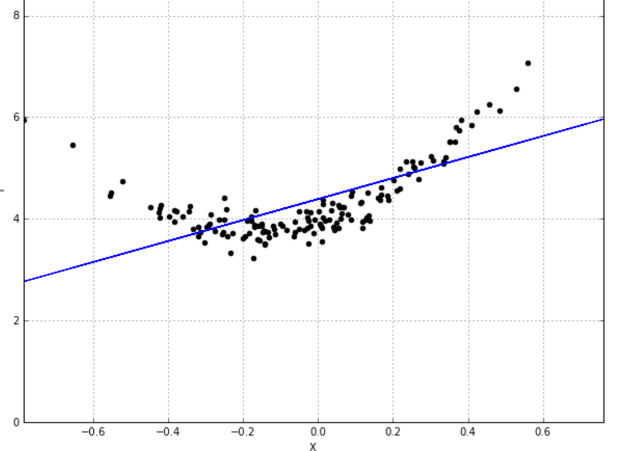
\includegraphics[scale=0.5]{problem} \pause

\begin{columns}
\begin{column}{7cm}

 $ y= \beta_0 + \beta_1 \cdot x + \beta_2 \cdot x^2 + \varepsilon$
\end{column}
\end{columns}
\end{frame}

%%%%%%%%%%%%%%%
\begin{frame}

\frametitle{Gaussov proces}

\begin{proposition} 
\alert{Slučajni proces} je zaporedje slučajnih spremenljivk $(X_t)_{t\ge0 } $.
\end{proposition}

\begin{proposition}
Slučajni proces $(X_t)_{t \in T } $ je \alert{Gaussov}, če je za katerokoli končno podmnožico $ F \subset T$, slučajni vektor $ X_F := (X_t)_{t \in F}$ (večrazsežno) normalno porazdeljen. 
\end{proposition}

Drugače: Slučajni proces je Gaussov, če je za vsak vektor neodvisnih spremenljivk $x$, vrednost funckije $f(x)$ porazdeljena po normalni (Gaussovi) porazdelitvi.
\end{frame}


%%%%%%%%%%%%%%%
\begin{frame}

\frametitle{Standardni linearni model}

Standardni linearni model regresije z Gaussovim šumov
\begin{enacba}
$$ f(x) = x^\mathsf{T} w, ~~~~~~  y= f(x) + \epsilon, $$
\end{enacba}

\begin{itemize}
\item $x$ vhodni vektor
\item $w$ vektor uteži/parametrov
\item $f$  funkcija
\item $y$ opazovana izhodna (ciljna) vrednost
\end{itemize}

Predpostavimo: $$ \epsilon \sim \mathcal{N}(0, \sigma_{n}^2).$$

\end{frame}


%%%%%%%%%%%%%%%
\begin{frame}

\frametitle{Verjetnostna gostota}

\begin{equation} 
\begin{split}
 p( y | X, w) &= \prod\limits_{i=1}^{n} p(y_{i} | x_{i}, w) = \prod\limits_{i=1}^{n} \frac{1}{\sqrt{2\pi} \sigma_{n}} exp(-\frac{ (y_{i}- x_{i}^\mathsf{T} w)^2}{2 \sigma_{n}^2})  \\
 &=\frac{1}{ (2\pi \sigma_{n}^2 )^{n/2}} exp( - \frac{1}{2\sigma_{n}^2}|y - X^\mathsf{T} w |^2)  
 \sim \mathcal{N}( X^\mathsf{T} w, \sigma_{n}^2 I).
\end{split}
\end{equation}


\begin{enacba} 
Predpostavimo: $ w \sim \mathcal{N}(0, \Sigma_{p}).$
\end{enacba}

\end{frame}

%%%%%%%%%%%%%%%
\begin{frame}

\frametitle{Posterior}
Sklepanje v Bayesovem linearnem modelu temelji na posteriorni porazdelitvi nad utežmi, izračunanimi po Bayesovem pravilu,
\begin{equation} 
posterior = \frac{verjetje \cdot prior}{robno~verjetje},   ~~  p(w|y,X) = \frac{p(y|X,w) \cdot p(w)}{p(y|X)}.
\end{equation}

Robno verjetje je neodvisno od uteži in podano kot

\begin{equation}
p(y|X) = \int p(y|X,w) p(w) dw.
\end{equation}

\end{frame}

%%%%%%%%%%%%%%%
\begin{frame}

\frametitle{Sorazmernost}

\begin{proposition} Pravimo, da je funkcija $f$ \alert{sorazmerna} $g$, če je $f(x)=k \cdot g(x)$ za poljubno konstanto $k$, neodvisno od $x$. Označimo $ f \propto g$.
\end{proposition}

$ p(w|X,y) = \frac{p(y|X,w) \cdot p(w)}{p(y|X)} $

\begin{equation}
\begin{split}
p(w| X,y) & \propto exp ( - \frac{1}{2 \cdot \sigma_{n}^2}( y- X^\mathsf{T} w)^\mathsf{T} (y - X^\mathsf{T} w)) \cdot exp(- \frac{1}{2} w^\mathsf{T} \Sigma_{p}^{-1}w) \\
& \propto exp (- \frac{1}{2}(w - w^*)^\mathsf{T} (\frac{1}{ \sigma_{n}^2} X X^\mathsf{T} + \Sigma_{p}^{-1}) (w-w^*)),
\end{split}
\end{equation}

kjer $w^* =  \sigma_{n}^{-2} (  \sigma_{n}^{-2} X X^\mathsf{T} + \Sigma_{p}^{-1})^{-1}Xy$. 

\end{frame}
%%%%%%%%%%%%%
\begin{frame}
\frametitle{Napovedi}
$ p(w| X,y) \propto exp (- \frac{1}{2}(w - w^*)^\mathsf{T} (\frac{1}{ \sigma_{n}^2} X X^\mathsf{T} + \Sigma_{p}^{-1}) (w-w^*)) $

$p(w |X,y) \sim \mathcal{N}(w^*, A^{-1})$


Da bi naredili napovedi za testni primer, povpečimo vse možne vrednosti parametra, utežene z njihovo posteriorno verjetnostjo.
Tako dobimo napovedno porazdelitev za $ f^{*}$ pri danem $x^{*}$.

\begin{equation}
\begin{split}
 p( f^* | x^*, X,y) &= \int p(f^* | x^*, w) \cdot p(w| X, y) dw  \\
 &= \mathcal{N}(\frac{1}{ \sigma_{n}^2} (x^*)^\mathsf{T} A^{-1} X y, (x^*)^\mathsf{T} A^{-1} x^*) 
 \end{split}
\end{equation}

\end{frame}


%%%%%%%%%%%%%%%%%%
\begin{frame}

\frametitle{Pogled iz prostora funkcij}

Gaussov proces $f(x)$ je določen s funkcijo matematičnega upanja $m(x)$ in kovariančno funkcijo $k(x, x')$, kjer sta:
\begin{itemize}
\item $ m(x) = E[ f(x) ] $, 
\item $ k(x, x') = E[ (f(x) - m(x)) (f(x')-m(x')) ] $.
\end{itemize}

Pišemo: $ f(x) \sim \mathcal{GP}(m(x), k(x,x'))$.
\end{frame}

%%%%%%%%%%%%%
\begin{frame}
\frametitle{Pogled iz prostora funkcij}

\begin{proposition}\alert{Marginalization property} { Če GP določa $ (y_{1}, y_{2})  \sim  \mathcal{N}(\mu, \Sigma) $, 
potem enolično določa tudi $y_{1} \sim  \mathcal{N}(\mu_{1}, \Sigma_{11})$, kjer je
$\Sigma_{11}$ pripadajoča podmatrika matrike $\Sigma$. }
\end{proposition}

%zmanjšanje množice ne spremeni porazdelitve, zato ni potrebno delati na neskončnem ali velikem prostoru (to ne vem če naj vključim gor)

\end{frame}

%%%%%%%%%%%%%%%%%%%%%%%%%%%%%%%%
\begin{frame}
\frametitle{Eksponentna kovariančna funkcija}

\begin{enacba}
 ~ ~ $cov(f(x_{p}), f(x_{q})) = k((x_{p},x_{q}) = exp( - \frac{1}{2} |x_{p} - x_{q}|^2).$
\end{enacba}
\begin{itemize}
\item Izberemo neko število vhodnih točk $X_{*}$ in zapišemo pripadajočo kovariančno matriko 
\item Potem generiramo slučajni normalni vektor z novo kovariančno matriko

\begin{equation} 
f_{*} \sim \mathcal{N}(0, K(X_{*}, X_{*})),
\end{equation}

\item ... in narišemo generirane vrednosti kot funkcijo vhodnih podatkov. 
\end{itemize}

\end{frame}


%%%%%%%%%%%%%%%%%%%%%%%5
\begin{frame}
\frametitle{Generiranje normalnih vzorcev}
\textbf{Generiranje normalnih vzorcev} \\
Za ustvarjaje vzorcev $ x \sim \mathcal{N}(m,K) $, s poljubnim povprečjem $m$ in kovarianco $K$ uporabimo t.i. Gaussov generator (ki je na voljo v mnogih programskih okoljih) in nadaljujemo na naslednji način: 
\begin{enumerate}
\item Izračunamo razcep Choleskega $L$ pozitivno definitne simetrične kovariančne matrike $K=LL$, kjer je $L$ spodnje-trikotna. 
\item Generiramo $ u \sim \mathcal{N}(0,I). $
\item Izračunamo $x= m+ Lu$, ki ima želeno porazdelitev s povprečjem $m$ in kovarianco $K$. 
\end{enumerate}


\end{frame}

%%%%%%%%%%%%%
\begin{frame}
\frametitle{Primer}
\begin{figure}[h]
\centering
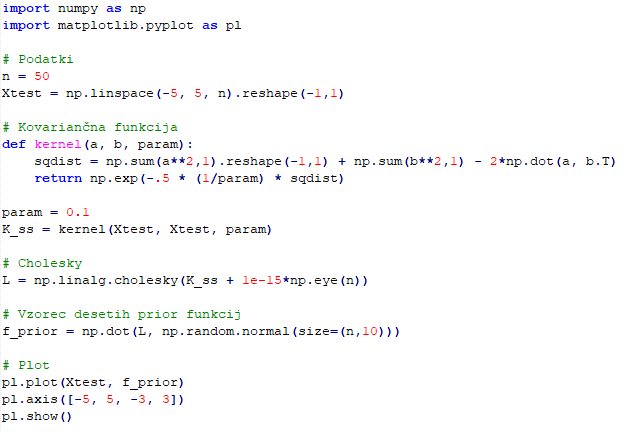
\includegraphics[width=1\textwidth]{python1}
\end{figure}

\end{frame}


%%%%%%%%%%%%%
\begin{frame}

\begin{figure}[h]
\caption{Primer 10 naključnih funkcij iz GP apriori}
\centering
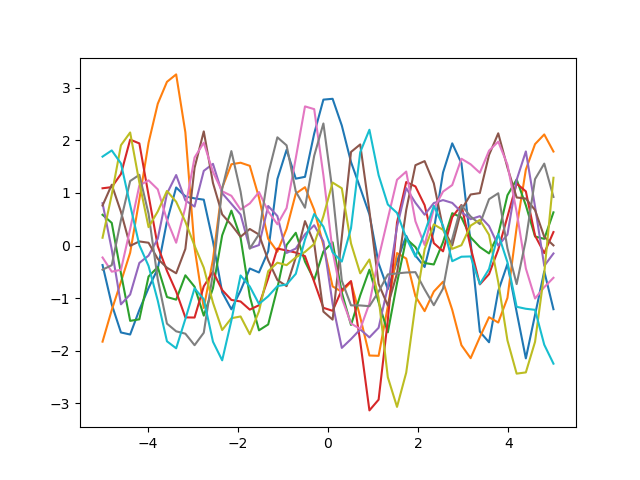
\includegraphics[width=1\textwidth]{10prior}
\end{figure}

\end{frame}

%%%%%%%%%%%%%
\begin{frame}
\frametitle{Znanje o funkciji, ki ga zagotavljajo vhodni učni podatki}
Najprej bomo obravnavali preprost poseben primer, kjer bodo opazovanja brez šuma, 
torej $ \{ (x_{i}, f_{i}) | i = 1, \ldots , n\}$.

Skupna porazdelitev učnih izhodov $f$ in testnih izhodov $f_{*}$, glede na apriori je
\begin{equation}
\begin{bmatrix}
f\\ 
f_{*}
\end{bmatrix}
\sim \mathcal{N} ( 0, 
\begin{bmatrix}
K(X,X) & K(X,X_{*}) \\ 
K(X_{*},X) & K(X_{*},X_{*})
\end{bmatrix})
\end{equation}
Da dobimo posteriorno porazdelitev funkcij, moramo omejiti skupno apriori porazdelitev tako, 
da bo vsebovala le funkcije, ki se prilegajo oz. vsebujejo opazovane vhodne točke. 

\end{frame}

%%%%%%%%%%%%%
\begin{frame}

\begin{izrek} Naj je $ \begin{bmatrix}
x\\ 
y
\end{bmatrix} $ normalno porazdeljen vektor
\begin{equation}
 \begin{bmatrix}
x\\ 
y
\end{bmatrix} \sim \mathcal{N}(\begin{bmatrix}
\mu_{x}\\ 
\mu_{y}
\end{bmatrix}, \begin{bmatrix}
A & C\\ 
C^\top & B
\end{bmatrix}) 
\end{equation}
potem sta \textbf{robna} porazdelitev $x$ in \textbf{pogojna} porazdelitev $x$ glede na $y$ enaki

\begin{equation}
\begin{split}
& x \sim \mathcal{N} (\mu_{x}, A) \\
& x|y \sim \mathcal{N} (\mu_{x} + CB^{-1}(y-\mu_{y}), A-CB^{-1}C^\top).
\end{split}
\end{equation}
\end{izrek}

\end{frame}
%%%%%%%%%%%%%%%%%%%%%
\begin{frame}

Če upoštevamo izrek dobimo porazdelitev posteriori funkcij

\begin{equation}
\begin{split}
f_{*} |( X_{*}, X, f ) ~ \sim ~ \mathcal{N} ( &K(X_{*},X) K(X,X)^{-1} f, \\
& K(X_{*},X_{*}) - K(X_{*},X)K(X,X)^{-1}K(X,X_{*})).
\end{split}
\end{equation}

Vrednosti funkcije $f_{*}$ dobimo s pomočjo prej opisanega postopka. 
\end{frame}
%%%%%%%%%%%%%%%%%%%%%%%%%%%%%
\begin{frame}
\begin{figure}[h]
\caption{Primer 10 naključnih funkcij iz GP posterior}
\centering
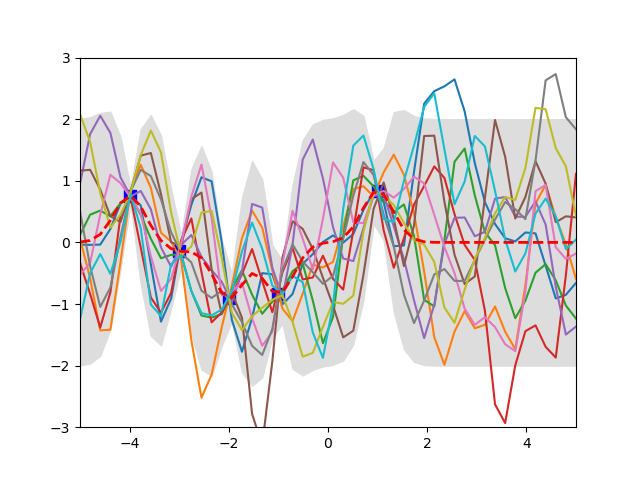
\includegraphics[width=1\textwidth]{10posterior}
\end{figure}

\end{frame}


%%%%%%%%%%%%%%%%%%%%%%%%%%%
\begin{frame}

\frametitle{Kovariančna funkcija}

Vrednost kovariančne funkcije $k(x_i, x_j)$ izraža korelacijo med posameznima izhodoma $f(x_i)$ in $f(x_j)$ modela, obravnavana kot dve medsebojno povezani naključni spremenljivki. 
\begin{itemize}
\item $ k(x_i, x_j) = E[ (f(x_i) - m(x_i)) (f(x_j)-m(x_j)) ] $.
\end{itemize}




\end{frame}

%%%%%%%%%%%%%%%%

\begin{frame}

\frametitle{Primerjava različnih kovarianc}
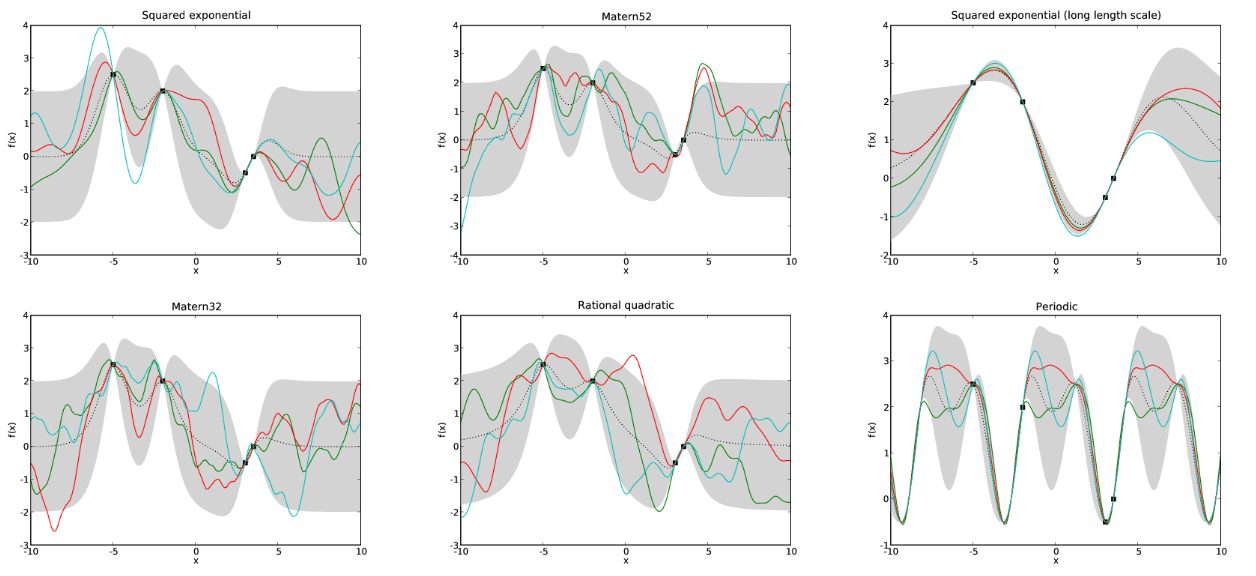
\includegraphics[scale=0.35]{kovariance}

\end{frame}
%%%%%%%%%%%%%%%%
\begin{frame}

\frametitle{GP model}

\begin{itemize}
\item \textbf{Predhodno znanje} (ang. \textit{prior}) odraža mnenje o preslikavi med vhodi in izhodi. Običajno predpostavlja gladkost.
\item \textbf{Posteriorno znanje} (ang. \textit{posterior}) dobimo, ko v model vključimo še končno število vhodno-izhodnih parov $(x_i, y_i)$.
Dobimo posteriorno porazdelitev za predikcijo modela. 
\item \textbf{Vhod} v GP model: posamezne vrednosti neodvisnih spremenljivk, zbrane v vhodnem vektorju x
\item \textbf{Izhod} iz GP modela: verjetnostna porazdelitev izhodne vrednosti $ f(x)$ pri danem vhodnem vektorju
\end{itemize}

\end{frame}

%%%%%%%%%%%%%%%%

\begin{frame}

\frametitle{Delo v nadaljevanju}
\begin{itemize}

\item Izbira kovariančne funkcije je ključnega pomena za delovanje GP modela.
\item Empirični del diplomske naloge

\end{itemize}


\end{frame}
%%%%%%%%%

\end{document}




